%! TEX root = diss.tex
\documentclass[../diss.tex]{subfiles}
\chapter{Preparation}

This chapter gives an overview of work that was completed before any code was
written. This includes theory surrounding parallel computing
(\autoref{sec:Parallel computing}) and computing shortest paths through matrix
multiplication (\autoref{sec:APSP algorithm}). It also includes the planning
the components of the implementation, done through making up assumptions
explicit (\autoref{sec:Parallel architecture assumptions}) and outline the
requirements (\autoref{sec:Requirements analysis}).  Lastly, I go over the
tools used (\autoref{sec:Choice of tools}) and the techniques used for
productive and manageable development (\autoref{sec:Software engineering}).

% Parallel computing (400 words?):
% * Flynn's taxonomy
% * Distributed memory model and alternative, Communication?
% * Massively parallel systems: Talk about supercomputers, grid computing,
%   sunway etc.
% * Evaluating a parallel algorithm, efficiency, communication-computation ratio
% Parallel computing {{{
\section{Parallel computing}%
\label{sec:Parallel computing}

% Where are you going?
% Why are you going there?
% And how are you going to get there?

We will now look at an overview of parallel computers. To design parallel
algorithms that utilize the computational resources as efficiently as possible,
we should be familiar with the landscape of parallel systems and their classifications. In this section, I will provide such an overview by classifying systems
according to how the streams of instructions are mapped onto data, what
hierarchies of memory are commonly used, and how this affects inter-processing-element communication. Additionally, we will discuss 
the scale at which parallelisation happens and cover metrics used for evaluating
how resource efficient a parallel algorithm is.

% Also define some metrics for evaluating how efficiently
%   the algorithm uses the computation reousrces available.

\subsection{Flynn's taxonomy}%
\label{sub:Flynn's taxonomy}

One way to classify parallel systems, is to look at how many streams of data
there are and how many sets of instructions the computer is operating with.
% What is a "stream" of data?

\begin{itemize}
    \item \ac{SISD} -- This is the same as sequential
        execution.
    \item \ac{MISD} -- Here, multiple sets of
        instructions are executed on the same input data. There are very few
        systems using this type of parallelism.
    \item \ac{SIMD} -- With this scheme, we apply
        the same set of operations to multiple sets of data simultaneously.
    \item \ac{MIMD} -- This is the most common
        type of parallelism in hardware. Multiple sets of instructions, possibly
        different, are applied to multiple sets of data at the same time.
\end{itemize}

Parallel systems typically use either \ac{SIMD} or \ac{MIMD}, where \ac{SIMD}
is common in \acp{GPU} and \ac{MIMD} is more often seen in systems where the
computation is spread among \acp{CPU}.

%There are also hybrid categories such as SPMD, relevant for supercomputer...

\subsection{Memory and communication}%
\label{sub:Memory and communication}

We can also classify parallel systems by how the memory is laid out. In systems
that use \textit{distributed memory}, each processor has its own private memory.
If communication between processors is required, there will be an interconnection
between the \acp{PE} that allows message passing. One common approach is an
interconnect network that can be arranged in a plethora of different
\textit{topologies}. If the topology is not fully-connected, the messages need
to be routed. A common network arrangement is the 2D Lattice Mesh, where there are
$p^2$ \acp{PE} connected to each of their four orthogonal neighbours and there
are cyclic connection that wrap around the edges.
In \textit{shared memory} systems, all the processors have access to a shared
address space. Multiple  \acp{PE} can communicate by reading and writing
to the same segment of memory, and locking mechanisms can be implemented to
prevent race conditions. % Fact check?

\subsection{Classes of  parallel computers}%
\label{sub:Classes of  parallel computers}

By looking at the extent to which the system supports parallelism and at the
physical distance between the \acp{PE}, we create further classifications.
In \textit{multi-core processors}, we refer to the \acp{PE} as \textit{cores}
and have several of them on the same chip. The cores execute in \ac{MIMD}-fashion
and there are typically both local memory for each core as well as some shared
memory between cores, that can be used for communication.
In \acp{MPP}, we often have many thousands of processors, interconnected through
a specialised network. An example is the Sunway TaihuLight supercomputer
\cite{sunway}.
There is also a wide class of computers known as \textit{distributed computers},
where the \acp{PE} communicate over a network, such as the Internet.
% TODO: cite Wikipedia?


\subsection{Evaluating performance}%
\label{sub:Evaluating performance}

A simple performance metric is the elapsed time, which works well when comparing
two different computers. However, it is not very useful when evaluating how 
efficiently
an algorithm exploits the parallelism available on a given system. For this,
the \textit{speed-up} is more useful:
\begin{equation}
    S_p = \frac{T_1}{T_p},
\end{equation}
where $T_1$ is the required time to solve the problem on a single
processor and $T_p$ is the elapsed time when executing the parallel algorithm
on $p$ processors.

Another useful metric is the \textit{parallel efficiency}, which is defined as
\begin{equation}
    \varepsilon = \frac{T_1}{p T_p} = \frac{S_p}{p}.
\end{equation}
The parallel efficiency ranges from 0 to 1, where $\varepsilon  =1$, means
we have a perfect linear speed-up where no
computation power is wasted when executing the algorithm on our parallel system.

Both of these metrics do not take into account the speed-up lost from the algorithm
having a serial part that cannot be parallelised. To incorporate this,
Amdahl's law or Gustafson's law have been used  \citep{parallelPerformance}.
However, the parallel algorithms developed in this project to solve \ac{APSP}
have a negligible serial part if we ignore the time required to read the input
and print the result. I will therefore not use these laws in evaluation.

In practice, what prevents linear speed-up is the \textit{communication cost} the
algorithm incurs while running on the parallel system. This can include both
\acp{PE} needing to idle while they wait for data to be ready or they are
waiting for some data to be transferred. % TODO: aren't these the same?
Another metric is therefore the ratio between computation and communication,
where a high ratio means we use our resources efficiently. We let
$T_p = \frac{T_{communication}+T_{computation}}{p}$, where $T_p$ is the time spent
on executing the parallel algorithm, where the sum of the costs are split up
into communication and computation costs. To execute a similar algorithm on a serial machine, we would avoid all the communication cost, but would still need to
do all the computation, so $T_1=T_{computation}$\footnote{
    This is assuming we are not using a completely different algorithm
    when solving the problem serially.
}.
We can relate this with the parallel
efficiency:
\begin{equation}%
\label{eq:parallel-efficiency}
    \varepsilon = \frac{T_1}{p T_p} = \frac{T_{computation}}{T_{computation}+T_{communication}}
\end{equation}
It is also easier to measure this ratio of computation.

% TODO: All of the above is very poorly worded. Redo this!
% DONE: write from here, about communication and computation ratio, time where
%  no useful work is done, stalling, waiting for data etc., SIMD masked computation


% }}}

% APSP algorithm (400 words?):
% * Mention known algorithms like Dijkstra, Floyd-Warshall, not very parallisable
% * MatMul highly parallisable and can be used
% * Repeated matrix squaring
% * Fox otto and Cannon's algorithm
% * Some more words here
% APSP algorithm {{{
\section{APSP algorithm}%
\label{sec:APSP algorithm}

% TODO: Find citation for dijkstra overhead?
% TODO: Look at implementation chapter, and add whatever details used there, such
%       as the distance product....
%       After this, we can create the introduction paragraph

% * What is a `distance product`, and explain concept of MatMul on the semiring

The main algorithm of the dissertation is based on matrix multiplication and
solves a problem in graph theory. By going through the notation and definitions
I will be using, as well as discussing alternative approaches to parallelising
\ac{APSP}, we can better understand the \ac{MatSquare} algorithm.
Throughout the dissertation, we consider graphs on the form $G=(V,E,w)$, where we have a set $V$ of $n$ vertices and a set
$E$ of edges and each edge $e \in E$ has a non-negative weight $w(e)$ assigned
to it. The \ac{APSP} problem concerns finding the \textit{shortest path} between
each pair of vertices.

\subsection{Parallelisation}%
\label{sub:Parallelisation}

There are many widely-used algorithms for efficiently solving the
\ac{SSSP} problem, such as Dijkstra's algorithm, Bellman-Ford and A$^*$-search.
If we have fewer than $n$ \acp{PE}, a trivial parallelisation for solving \ac{APSP}
is to run one of these algorithms on each \ac{PE}, distributing the sources.
However, this approach does not use our parallel resources efficiently if we have
more than $n$ \acp{PE}. To exploit this, we must either consider other algorithms
or parallelise parts of the \ac{SSSP} computation in one of these algorithms.
Parallel versions of these algorithms have been developed in the past
\cite{parallelDijkstra,astar},
% TODO: citation needed
but they incur a significant overhead. I have therefore decided to use a new
algorithm based on matrix multiplication, a highly paralleliseable task,
instead.

\subsection{Repeated matrix squaring}%
\label{sub:Repeated matrix squaring}

Matrix multiplication usually happens over the \textit{semiring}\footnote{See
appendix \autoref{sec:Abstract algebra}.} $(\mathbb{R},+,\cdot)$.
However, we replace addition with multiplication and  multiplication by the
$\min$-operator, resulting in the tropical semiring $(\mathbb{R}^*, \cdot,\min)$,
where we define $\mathbb{R}^* \triangleq \mathbb{R}\cup\{\infty\}$. When doing
matrix multiplication over this algebra, we perform an operation called
the \textit{distance product}.
\begin{definition}
    The distance product of two matrices, $A$ and $B$, whose entries $(i,j)$
    give the length of the shortest path $i \rightsquigarrow j$ of length
    exactly $n$ and $m$, respectively, is a matrix $M$ whose entries $(i,j)$
    are given by
    \begin{equation}%
    \label{eq:distanceProduct}
        M_{i,j} = [A \otimes B]_{i,j} = \min_{k}\left( A_{i,k} \cdot B_{k,j}\right).
    \end{equation}
    Each entry $M_{i,j}$ then gives the distance of the shortest path
    $i \rightsquigarrow k \rightsquigarrow j$ of length $n+m$.
\end{definition}
If we let $W$ be the adjacency matrix, where each entry $(i,j)$ is the weight
of edge $(i,j)$ and $\infty$ if $(i,j) \not\in E$, then computing the distance
product of $W$ with itself $k$ times will give a matrix containing the length
of shortest paths of length $k$.
If we add a self-loop to each vertex with weight 0, and compute $W^n$, the matrix
will contain the shortest-distances between all pairs of nodes that are of length
at most $n$, i.e. the shortest path (because it cannot be longer).
A more efficient way to compute this is by squaring
 $W$ $\lceil \log_2 n \rceil$ times. This
% TODO: explain abbreviation better
is the idea behind the \ac{MatSquare} algorithm that I explain in
\autoref{sec:APSP via repeated matrix-squaring}.

% }}}

% Parallel simulation (200-300 words?):
% * Having review above algorithm and hardware for parallel computing, decide
%   what "model of computation" to use.
% * Don't have access to this, and don't want to use GPU because ...
% * List all the assumptions made, e.g. message passing because FoxOtto ...
% * Why MIMD:
%    * SIMD is the most suitable for _standard_ MatMul because repeated operation
%    However, we are using a modification of that where also computation for
%    predecessor pointer, and done over min-plus semiring, so none of that
%    functionality peformed if don't branch. With SIMD, we mask instruction if have
%    branches, which wastes computation. More room for gain if assume MIMD
%    * Additionally, MIMD most common in message passing systems, and SIMD systems
%    like GPUs typically use shared-memory, not distributed.
%    * (Also possible extensions, like FW, ...?) <- not very good argument
% Parallel simulation {{{
\section{Parallel architecture assumptions}%
\label{sec:Parallel architecture assumptions}

% Note: The idea behind this section is tying everything together, **why**
%   have we made all these decisions on our parallel system...

In this section, I will list the assumptions behind the parallel system that
will be simulated. For the implementation to go as smoothly as possible and the
timing evaluation to be applicable, it is important to have a clear and
well-defined parallel system in mind. As we saw in \autoref{sec:Parallel computing}, there are many classes of parallel systems. We will hone in on a particular
parallel system by making assumptions about its model of memory, its execution,
and how it supports message-passing.

% Regardless of system, it should have a configurable number of \acp{PE}, and
% this number can be very high as we might want to evaluate performance with
% many.

\paragraph{Memory model}%
\label{par:Memory model}

I assume a fully-distributed memory model, where each \ac{PE} has its own private
memory and no address space is shared between different \acp{PE}. To allow
coordination, a message-passing interface is also assumed. This model scales well
with a very large number of \acp{PE}, compared with shared-memory systems where
the memory system becomes a bottleneck when the number of \acp{PE} that share
the same memory are in the 1000s. I also assume that each \ac{PE} has sufficient
private memory to store the data it will be working on, but I will not abuse this
to store a copy of the input on each \ac{PE}.

\paragraph{MIMD execution}%
\label{par:MIMD execution}
I also assume that each \ac{PE} runs independently of the others, so their
computation might not be synchronised even if they all execute the same algorithm.
I have decided to assume this model of execution over \ac{SIMD} for the
following reasons:
\begin{itemize}
    \item In distributed-memory systems with message passing, \ac{MIMD} is the
        most common, whereas \ac{SIMD} is most-often seen in shared-memory
        systems. Simulating \ac{MIMD} thus gives more realism.
        % TODO: for this to make sense, add details on masking and on predecessor
        %    above in prepearation
    \item With \ac{SIMD}, if two or more \acp{PE} take different branches,
        computation is masked with \texttt{NOP}-instructions. This wastes
        computation resources, and is difficult to simulate. In standard
        matrix multiplication, there are no branches, but we are implementing
        a alternative matrix multiplication algorithm for the
        $(\mathbb{R}^*,\cdot,\min)$ semiring, where we also have computation for
        finding the predecessors. This introduces possibly large branches in
        our inner-loop.
    % flexibility?
\end{itemize}
In the initial plan for the project, I set out to use a na{\"i}ve simulation
of \ac{SIMD}, where I would just average the computation time of each \ac{PE}.
The change to a more realistic \ac{MIMD} execution model was an extension that
was not planned for in the project proposal.

\paragraph{Message passing}%
\label{par:Message passing}
The \acp{PE} are interconnected through point-to-point links, arranged in
some connected network topology. I will assume the \acp{PE} are laid
out in a square lattice arrangement because the problem of matrix multiplication
maps nicely to this. Additionally, the Fox-Otto algorithm assumes row-broadcast
highways, so I will also assume these are available. Further, I will assume that
each broadcast-highway as well as each point-to-point link can only be used to
carry one message at a time. The messages are also delivered \textit{in-order}.

The time it takes to send a message $m$ from \ac{PE} $i$ to \ac{PE} $j$ only
depends on the size of $m$, the latency and bandwidth of the links, and the
value of some fixed function $d(i,j)$, that depends on the interconnect topology.
I will also assume the latency and bandwidth are the same for all messages sent.
I also assume some fixed latency and bandwidth for the broadcasting.

% }}}


% Requirements analysis (500 words)
% Requirements analysis {{{
\section{Requirements analysis}%
\label{sec:Requirements analysis}

% Where are you going? Why are you going there? And how are you going to get there?
We will now look at the main components to be implemented, and what their
functional requirements are. To make implementation as smooth as possible, it
is important to know beforehand what the different components will do and how
they interface with other components. This will also make modular development
easier as we only need to focus on one component and its interface at a time.

\paragraph{Parallel system simulation}%
\label{par:Parallel system simulation}

Since I do not have access to a physical system fitting the
properties described in \autoref{sec:Parallel architecture assumptions},
I will simulate one. The main requirements of this is:
\begin{itemize}
    \item Configurable number of \acp{PE} and topology
    \item Simulation exploits inherent parallelism on system it is executed on,
        such that it's as efficient as possible
    \item There is a simple, yet expressive, interface for describing the
        computation to be performed at each \ac{PE}, where the programmer has
        access to methods such as \texttt{send}, \texttt{receive},
        \texttt{broadcastRow} etc., and can retrieve its position in the grid with
        \texttt{i} and \texttt{j}. 
        % ?
        With such an interface, other algorithms like parallel Floyd-Warshall
        can also be implemented.
    \item There is an interface for distributing input data among the \acp{PE}
        as well as retrieving the result.
    \item The computation time is measured during \ac{PE} execution, and
        communication time is estimated according to the message passing model in 
        the assumed architecture.
    % TODO: add something more about how should comply with assumed arch?
\end{itemize}

\paragraph{Graph datasets}%
\label{par:Graph datasets}

To evaluate the performance scaling of our algorithms, we will need a large set
of different input graphs, covering a sufficiently large space of sizes. Ideally,
these graphs should have similar characteristics as well as resemble real-world
graphs like road networks as this is a primary usage of our \ac{APSP} algorithm.

We also need a \textit{graph input} component that can read the graphs from file
and transform them into a suitable format to pass as input to the \ac{APSP}
algorithm.

\paragraph{APSP algorithm}%
\label{par:APSP algorithm}

We can summarise the requirements of this component as:
\begin{itemize}
    \item Given an input graph $G$, it can compute the shortest paths between
        each pair of nodes in $V$. This computation is done by using the
        interface for the parallel architecture simulation.
    \item After this computation, each path $i \rightsquigarrow j$ can be
        reconstructed.
    \item This computation can also happen when the parallel arcitecture is
        configured to have fewer \acp{PE} than there are vertices in the
        graph (extension).
\end{itemize}

\paragraph{Graph compressor (extension)}%
\label{par:Graph compressor}

The input graph can be passed to this module and a new ``equivalent'', but with
all the 2-degree-nodes removed is returned. Additionally, after solving
\ac{APSP} on this compressed graph, we can pass the solution back to the
graph compressor to reconstruct \ac{APSP} solutions on the original graph.
% TODO: rephrase...

% }}}

% Choice of tools (200 words)
% * Java, OOP, modularity benefits
% * GitHub, CI to check builds when push
% * JUnit4, unit testing framework for Java
% * Python for data analysis and plotting
% Choice of tools {{{
\section{Choice of tools}%
\label{sec:Choice of tools}

We will now go over various existing software, programming languages
and services that can aid the development. When developing and testing
a parallel program, there are many already built tools and utilities that
handle a lot of the work, such as high-level synchronisation classes or
unit testing frameworks. By using these tools, we can spend more time on the
core parts of the project, like creating the simulation and developing the
\ac{MatSquare} algorithm.

\subsection{Programming languages and libraries}%
\label{sub:Programming languages and libraries}

I chose Java for the implementation of the components of the project. The parallel
simulation has many modules that interact with each other, and implementation
is more manageable if these can be developed in isolation, abstracting away
their functionality. Additionally, code-reuse and dynamic polymorphism will be
important when implementing different algorithms for the parallel system's
interface. As such, and object-oriented language like Java, which makes following
these principles easier, is suitable. Additionally, Java is well-suited for
creating concurrent programs as it has built-in primitives for synchronisation as
well as classes for managing a large number of concurrent threads.

For testing, I use JUnit\footnote{\url{https://junit.org}}, which is a testing
framework for the \ac{JVM}. Since the code is modularised, this will allow me
to create well-organised unit tests for the different modules. To generate the
random graphs, I use the \texttt{NetworkX} library in Python, and these graphs
can also be visualised using a \texttt{ForceAtlas2} library.  For plotting my
evaluation results, I use python and modules like \texttt{pandas} and
\texttt{matplotlib}.

\subsection{Development, testing and revision control}%
\label{sub:Development, testing and revision control}

To easily manage different versions of the codebase, I will do revision control
with \texttt{git} and GitHub\footnote{\url{https://github.com/}}. I also set up
contiguous integration with  GitHub Workerflows, which compiles the project
every time I push a commit. This way, I can make sure the code is always in a
valid state and there are no syntax errors.  I will use my Acer Nitro Laptop,
running Ubuntu Linux 18.04 LTS, to both write and run all of my code. It has a
quad-core CPU (an Intel i5-8300H \@ 2.30~Ghz), 8~GB of RAM, and an NVIDIA GTX
1050 Mobile. The CPU supports running 8 threads concurrently, which means
parallelising the simulation itself will make a significant impact on the
simulation time. To write the Java code, I use the IntelliJ IDEA IDE to improve
the quality of the code and spend less time on getting the Java syntax right.

% }}}

% Starting point (100 words)
% Starting point {{{
\section{Starting point}%
\label{sec:Starting point}

\begin{table}[h]
\begin{center}
    \begin{tabular}{p{200pt}|p{230pt}}
        \textbf{Course} & \textbf{Relevance} \\
        \hline
        Object-Oriented Programming (OOP) & Principles behind
        writing OOP code and managing a large codebase \\
        Further Java & Some experience writing parallel programs \\
        Concurrent and Distributed Systems & Knowledge of concurrency concepts \\
        Computer Design & Knowledge of parallel systems \\
        Algorithms & Serial route-planning algorithms \\
    \end{tabular}
\end{center}
\caption[Tripos courses]{Courses from the Tripos and their relevance to my project.}
\label{tab:courses}
\end{table}

Many courses from the Computer Science Tripos have been useful for my project,
as seen in \cref{tab:courses}. The unit of assessment, Advanced Data Science,
has also been applicable when managing and visualising the timing data gathered
for the evaluation.

% }}}


% Software engineering (200?)
% Software engineering {{{
\section{Software engineering}%
\label{sec:Software engineering}

% TODO: disctintion between graph reader, and concept of input graphs is not
%    very clear in both above reqAnal and the diagram!
\begin{figure}
\begin{center}
    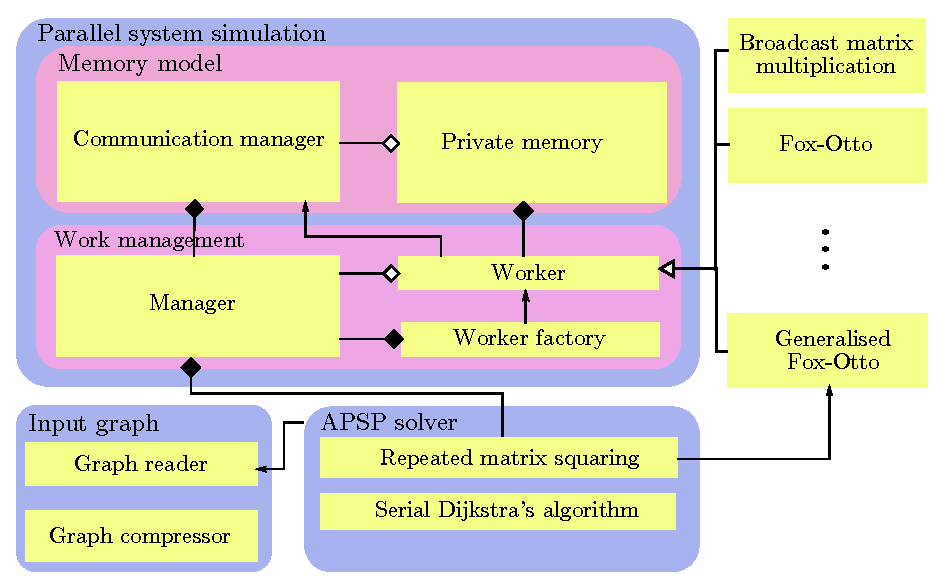
\includegraphics[scale=1]{figs/component-overview.pdf}
\end{center}
\caption{High-level overview of the implementation}
\label{fig:component-overview}
\end{figure}

In \autoref{fig:component-overview}, we see the high-level structure of the
implementation. This matches the requirements laid out in
\autoref{sec:Requirements analysis}; The requirements in each group can also be
associated with individual components. For example, allowing descriptions of
computation comes from the \texttt{Worker} interface, while access to communication
methods come from implementation of the communication manager. This sets up clear
work items and achievements to aim for during implementation.

I developed the parallel system simulation using the \textit{incremental build
model}. The simulator is very modular and the component dependencies form a
% TODO: acronym: DAG
directed acyclic graph, so implementation could happen by developing one module at
a time, and incrementally expanding the simulator.
I started implementation with the \texttt{Worker} and its private memory,
and tested its independent execution using various test-sub-classes. I then moved
onto incorporating communication methods such as \texttt{send} and
\texttt{broadcastRow} with the communication manager, which I tested using more
sub-classes of the \texttt{Worker} interface. After this, managing several workers
at a time, and handling their automatic creation, was implemented with the
\texttt{Manager} class and the worker factory, respectively. Then I incorporated
the communication manager. The functionality for timing the execution is
implemented using the \textit{decorator} pattern, so this could incrementally
be developed at any time after the parallel system simulation was done.

The higher-level components such as the simulation, the \ac{APSP} solver and
the input graph module were implemented according to the
\textit{iterative development model}. These components were fairly independent
as we could use a serial matrix multiplication algorithm instead of running code
on the parallel system. This allowed me to focus on one component at a time, as
well as separate testing.

% Incrementally make
% * parallel system simulation
% * dependencies one-directional, so can make one component at a time, made sure
%   to make clear interfaces such that when developing another module on top, only
%   need to think about interaction
% * Clear modularisation, so focus on one worker first, then develop communication
%   between them, then create manager to handle the execution and communication,
%   then build test workers classes, and then make repeated use the worker
% Iteratively:
% * The input graphs, graph reader seperate from simulation, additionally, can
%   detach MatSquare by using serial matrix multiplication routine instead of
%   manager

I followed proper software engineering techniques during development. Encapsulation and
modularisation were widely used and realised through use of immutability, access control
mechanisms and packaging my code. I also wrote exceptions and assertions throughout my
code where it was appropriate. I also used a coherent coding style and documented both
my methods and classes according to the Javadoc\footnote{\url{https://www.oracle.com/java/technologies/javase/javadoc-tool.html}} standard. The various components were also
unit-tested.

% }}}

% Summary
% Summary {{{
\section{Summary}%
\label{sec:Summary2}

In this chapter, I reviewed work done before code was written.
I presented a brief overview of different classes of parallel
systems and the concept behind the \ac{APSP} algorithm.
I also laid out the requirements for the different parts of the project,
emphasising the assumptions made about the parallel system to be simulated.
Then I outlined the choice of tools and techniques to be used during
development.

% }}}

% vim: foldmethod=marker
